% easychair.tex,v 3.4 2015/12/10

\documentclass{easychair}
%\documentclass[EPiC]{easychair}
%\documentclass[debug]{easychair}
%\documentclass[verbose]{easychair}
%\documentclass[notimes]{easychair}
%\documentclass[withtimes]{easychair}
%\documentclass[a4paper]{easychair}
%\documentclass[letterpaper]{easychair}

\usepackage{doc}

%use packages added by karla
\usepackage[utf8]{inputenc}
\usepackage[english]{babel}
\usepackage{color}
%use packages added by karla

% use this if you have a long article and want to create an index
% \usepackage{makeidx}

% In order to save space or manage large tables or figures in a
% landcape-like text, you can use the rotating and pdflscape
% packages. Uncomment the desired from the below.
%
% \usepackage{rotating}
% \usepackage{pdflscape}

% Some of our commands for this guide.
%
\newcommand{\easychair}{\textsf{easychair}}
\newcommand{\miktex}{MiK{\TeX}}
\newcommand{\texniccenter}{{\TeX}nicCenter}
\newcommand{\makefile}{\texttt{Makefile}}
\newcommand{\latexeditor}{LEd}

%\makeindex

%% Front Matter
%%
% Regular title as in the article class.
%
% \title{The {\easychair} Class File\\
%        Documentation and Guide for Authors%
% \thanks{Other people who contributed to this document include Maria Voronkov
%   (Imperial College and EasyChair) and Graham Gough (The University of
%   Manchester).}}

\title{Reconciling SCXML and Event-B Semantics}

% Authors are joined by \and. Their affiliations are given by \inst, which indexes
% into the list defined using \institute
%
% \author{
% Serguei A. Mokhov\inst{1}\thanks{Designed and implemented the class style}
% \and
%     Geoff Sutcliffe\inst{2}\thanks{Did numerous tests and provided a lot of suggestions}
% \and
%    Andrei Voronkov\inst{3}\inst{4}\inst{5}\thanks{Masterminded EasyChair and created versions
%      3.0--3.4 of the class style}
% }

\author{
Karla Morris\inst{1}
\and
Colin Snook\inst{2}
}

% Institutes for affiliations are also joined by \and,
\institute{
  Sandia National Laboratories, 
  Livermore, California, U.S.A.\\
  \email{knmorri@sandia.gov}
\and
   University of Southampton,
   Southampton, United Kingdom\\
   \email{cfs@ecs.soton.ac.uk}\\
 }

%  \authorrunning{} has to be set for the shorter version of the authors' names;
% otherwise a warning will be rendered in the running heads. When processed by
% EasyChair, this command is mandatory: a document without \authorrunning
% will be rejected by EasyChair

\authorrunning{}

% \titlerunning{} has to be set to either the main title or its shorter
% version for the running heads. When processed by
% EasyChair, this command is mandatory: a document without \titlerunning
% will be rejected by EasyChair

\titlerunning{}

\begin{document}

\maketitle

\begin{abstract}
  BLA BLA 
\end{abstract}

% The table of contents below is added for your convenience. Please do not use
% the table of contents if you are preparing your paper for publication in the
% EPiC series

\setcounter{tocdepth}{2}
{\small
\tableofcontents}

%\section{To mention}
%
%Processing in EasyChair - number of pages.
%
%Examples of how EasyChair processes papers. Caveats (replacement of EC
%class, errors).

\pagestyle{empty}

%------------------------------------------------------------------------------
\section{Introduction}
\label{sect:introduction}


% \begin{figure}[tb]
% 	\begin{centering}
% 	
\includegraphics[width=0.5\textwidth]{logoEC}
% 	\caption{EasyChair logo}
% 	\label{fig:easychair-logo}
% 	\end{centering}
% \end{figure}

\textcolor{red}{This section should focus on the motivation behind pursuing a scxml 
representation of our models, what are the benefits?}

SCXML is a general-purpose event-based state machine 
language that combines concepts from CCXML and Harel 
State Tables. Harel State Tables are included in UML. 
The concrete syntax for SCXML\footnote{http://www.w3.org/TR/scxml/} is based on XML. Hence, 
SCXML is an XML notation for UML style state-machines 
extended with an action language that is intended for 
call control features in voice applications.

%------------------------------------------------------------------------------

\section{Differences in Semantics}
\label{sect:diff}

\textcolor{red}{Differences in semantics between scxml and event-b}

\textcolor{red}{Elude to the reason for ignoring some of the scxml feature 
when it comes to the translation.}

\textcolor{red}{List the difference in the syntax of each representation (Short section)}

\begin{description}
\item [Refinement:]
Refinement is a central concept in iUML-B, detail is 
added in refinements by progressive hierarchical 
nesting. There is no refinement in SCXML.

\item [Transition firing:]
SCXML has equivalent hierarchical state constructs to 
iUML-B but differs significantly in the transition 
firing mechanism. In iUML-B transitions fire 
spontaneously when their guard (including source state) 
is true. In SCXML, transitions are triggered by the 
occurrence of some other event, which may be external 
or induced by the actions of another transition. 
In iUML-B if several transitions are simultaneously 
enabled one of the enabled transitions is non-
deterministically chosen for firing whereas SCXML has 
ordering rules to determine which transitions to fire 
next.

\item [Transition execution:]
When a particular SCXML transition fires it carries out 
a sequence of actions in particular order. For example 
a hierarchy of nested source states are exited (
performing exit actions) starting from the innermost 
one and working outwards. Presumably the order of 
taking actions is significant in SCXML (perhaps some of 
these actions could write to the same variable). In 

Event-B all actions of a transition are executed 
simultaneously in parallel by the elaborated event. It 
is not possible (i.e. not well-formed) for two of these 
actions to write to the same variable.
SCXML transitions can be designated ‘internal’, which 
prevents exiting and re-entering its source state in 
some cases. In SCXML target state can be omitted which 
results in a transition that does not change state (
this is different from a transition that exits a state 
and then re-enters the same state).
Neither of these features is supported in iUML-B since 

\item [Events:]
The meaning of event is very different between iUML-B 
and SCXML. In iUML-B transitions are sub-parts of 
events. In order for an event to be enabled for firing, 
all of its sub-parts (transitions) must be 
simultaneously enabled. This means that two different 
transitions with the same event can only fire at the 
same time and hence will never fire if they are sourced 
from different states of the same parent state-machine. 
In SCXML, events are triggers that enable transitions 
to fire. If two different transitions from different 
source states are both triggered by the same event, one 
may fire without the other if one source state is not 
active.

\item [Final States:]
The concept of a final state differs between iUML-B and 
SCXML. In SCXML a state machine (or parent state) may 
reside in a final state indicating that it is done and 
waiting for another transition to exit the parent 
state.  In iUML-B a final state is not a proper state 
of the parent state-machine. It is merely a notation 
for indicating that the state-machine is becoming non-
active. I.e. that the parent state is exiting. Hence 
any transitions that target a final state are part of a 
transition that leaves the parent state. For a ‘root’ 
state-machine the final state means that the state-
machine has been left completely and no state is active.

\item [Initial States:]
Initial states are similar to iUML-B. The transition 
from the initial state forms part of the actions to 
enter the parent state. However, the correspondence 
between incoming transitions to the parent state and 
initial transitions is more explicit in iUML-B. 
SCXML has another way to specify an initial state using 
an attribute of the state. In this case there is no way 
to add extra transition actions.
If no initial state is specified, the default is the 
first one in the document.
iUML-B allows different intial states for different 
incoming transitions. In SCXML this would be done by 
extending the transition into the substate.

\item [Entry/Exit Actions:]
SCXML includes the concept of entry and exit actions 
which are executed whenever a transition enters, resp. 
exits, the containing state. 
iUML-B does not current implement entry/exit actions,
but it is has been planned to add them.  This could be 
done as part of the work to support the iUMLB\_SCXML 
plugin, however, due to the extensive semantic 
differences between iUML-B and SCXML, it may be found 
that iUML-B entry/exit actions are not useful for 
supporting SCXML and a different solution is necessary.

\end{description}

%------------------------------------------------------------------------------

\section{Reconciling Semantics}
\label{sect:recon}

\textcolor{red}{Reconciling scxml semantics for event-b code generation.  
(Important, people will be interested)}

%------------------------------------------------------------------------------

\section{Extending SCXML}
\label{sect:extension}

\textcolor{red}{Methodology for adding required information to allow refinement, invariants,
guards, variable type declaration.}

%------------------------------------------------------------------------------

\section{Case Study}
\label{sect:caseS}

\textcolor{red}{Find a system that we can model and some how describe the benefits 
(e.g. model simplification) of using a specific syntax over the other.
	\begin{itemize}
		\item What model behavior can you capture with each semantic?
		\item What properties of the model are easier to simulate?
		\item Where do we introduce unnecessary complexity?
	\end{itemize}	
}

%------------------------------------------------------------------------------
\section{Conclusion}
\label{sect:concl}

Just to have a reference ~\cite{texniccenter}

%------------------------------------------------------------------------------
\section{Future Work}
\label{sect:future-work}


% \begin{figure}[tb]
%   \begin{centering}
%     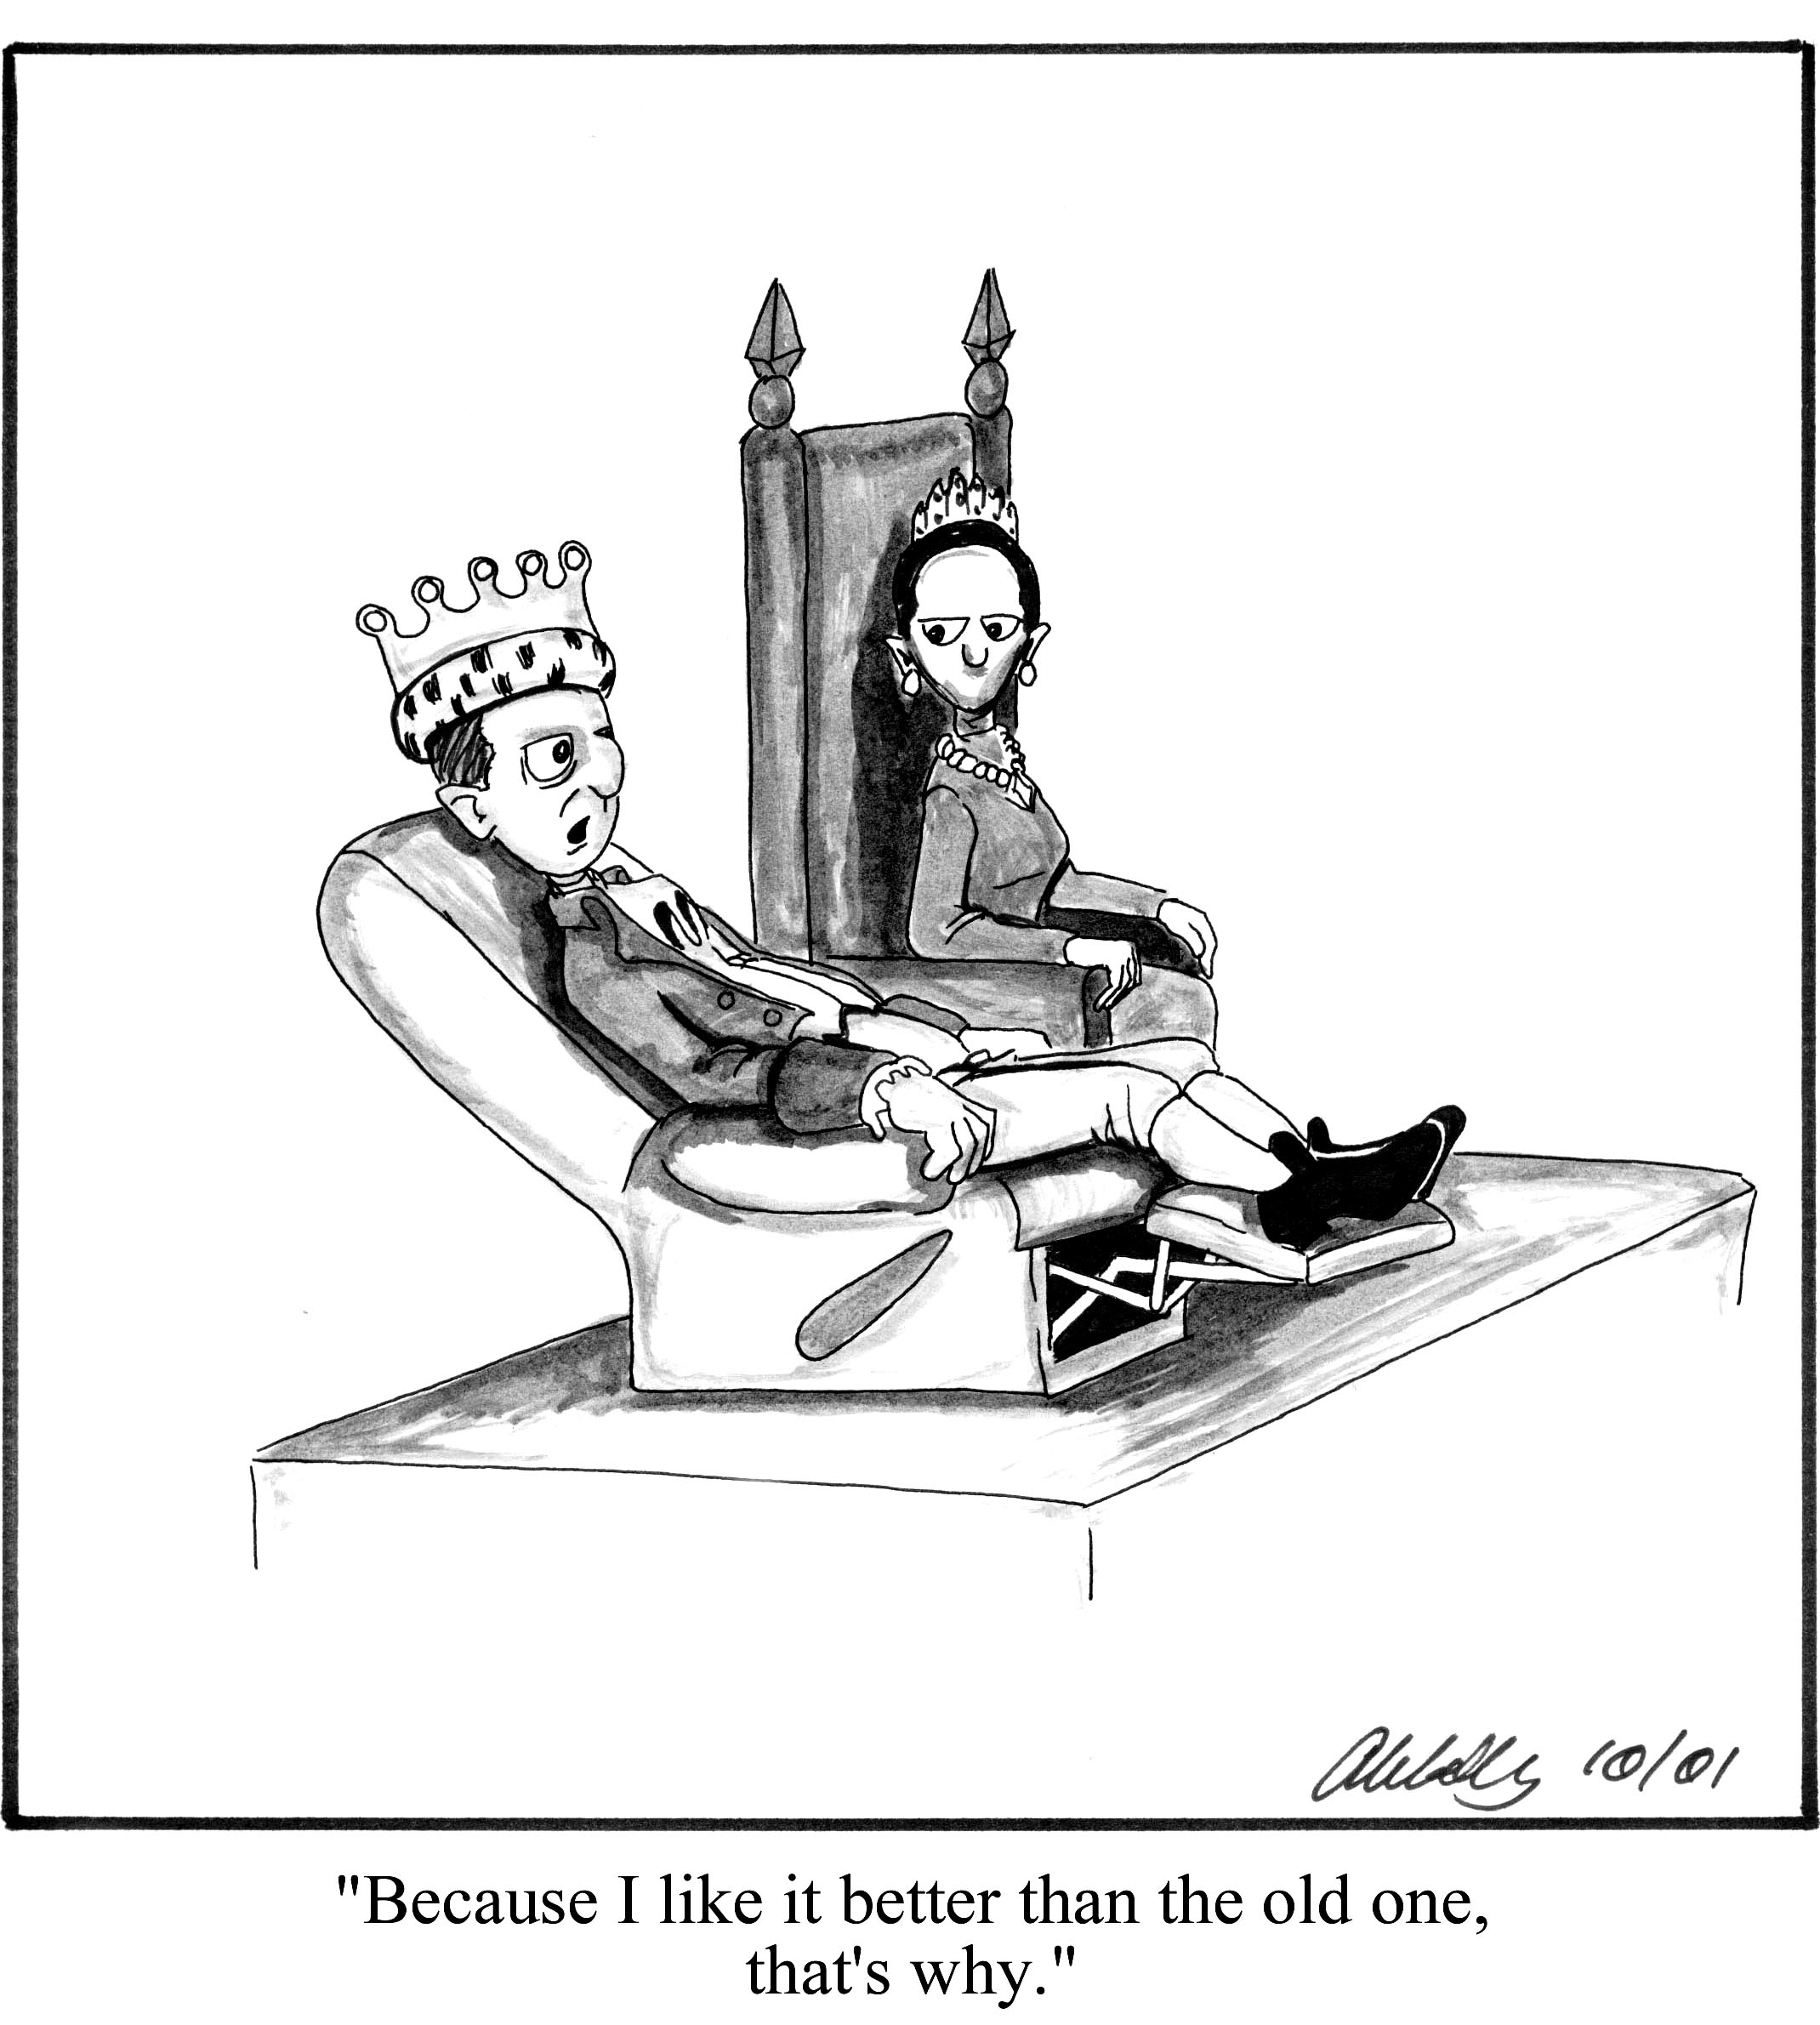
\includegraphics[width=0.5\textwidth]{throneEC.jpg}
%     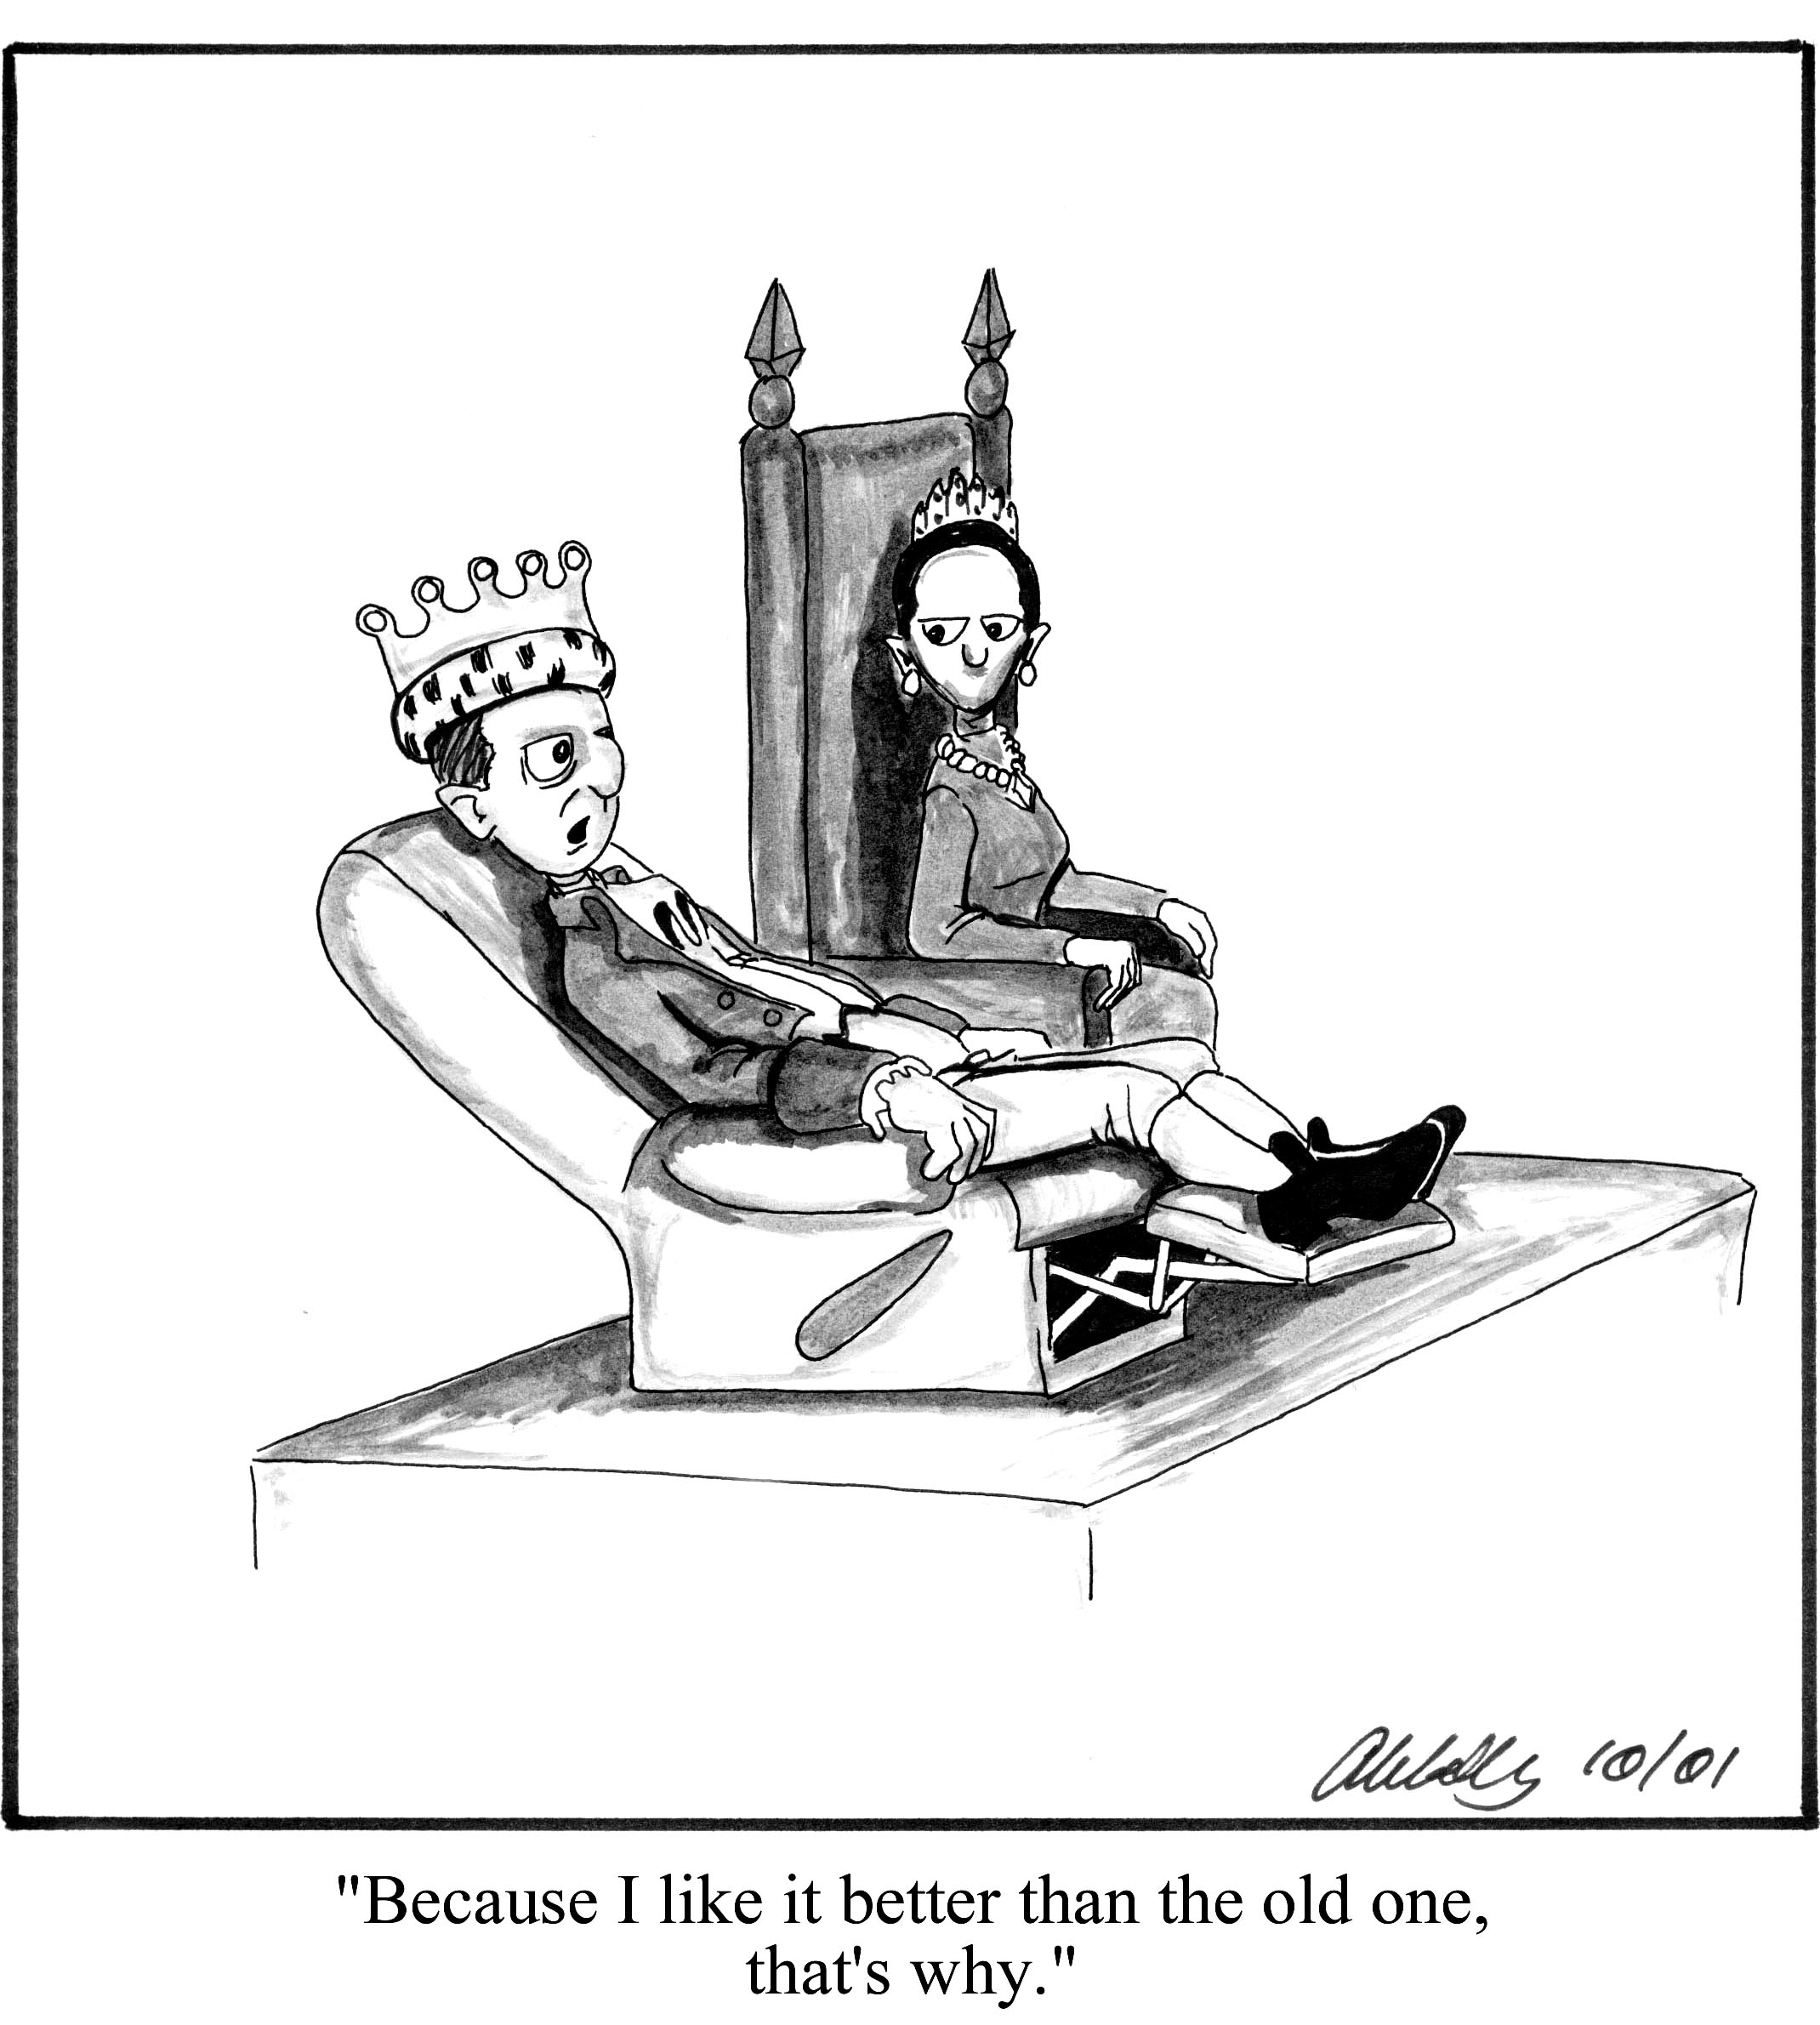
\includegraphics[width=0.3\textwidth]{throneEC.jpg}
%     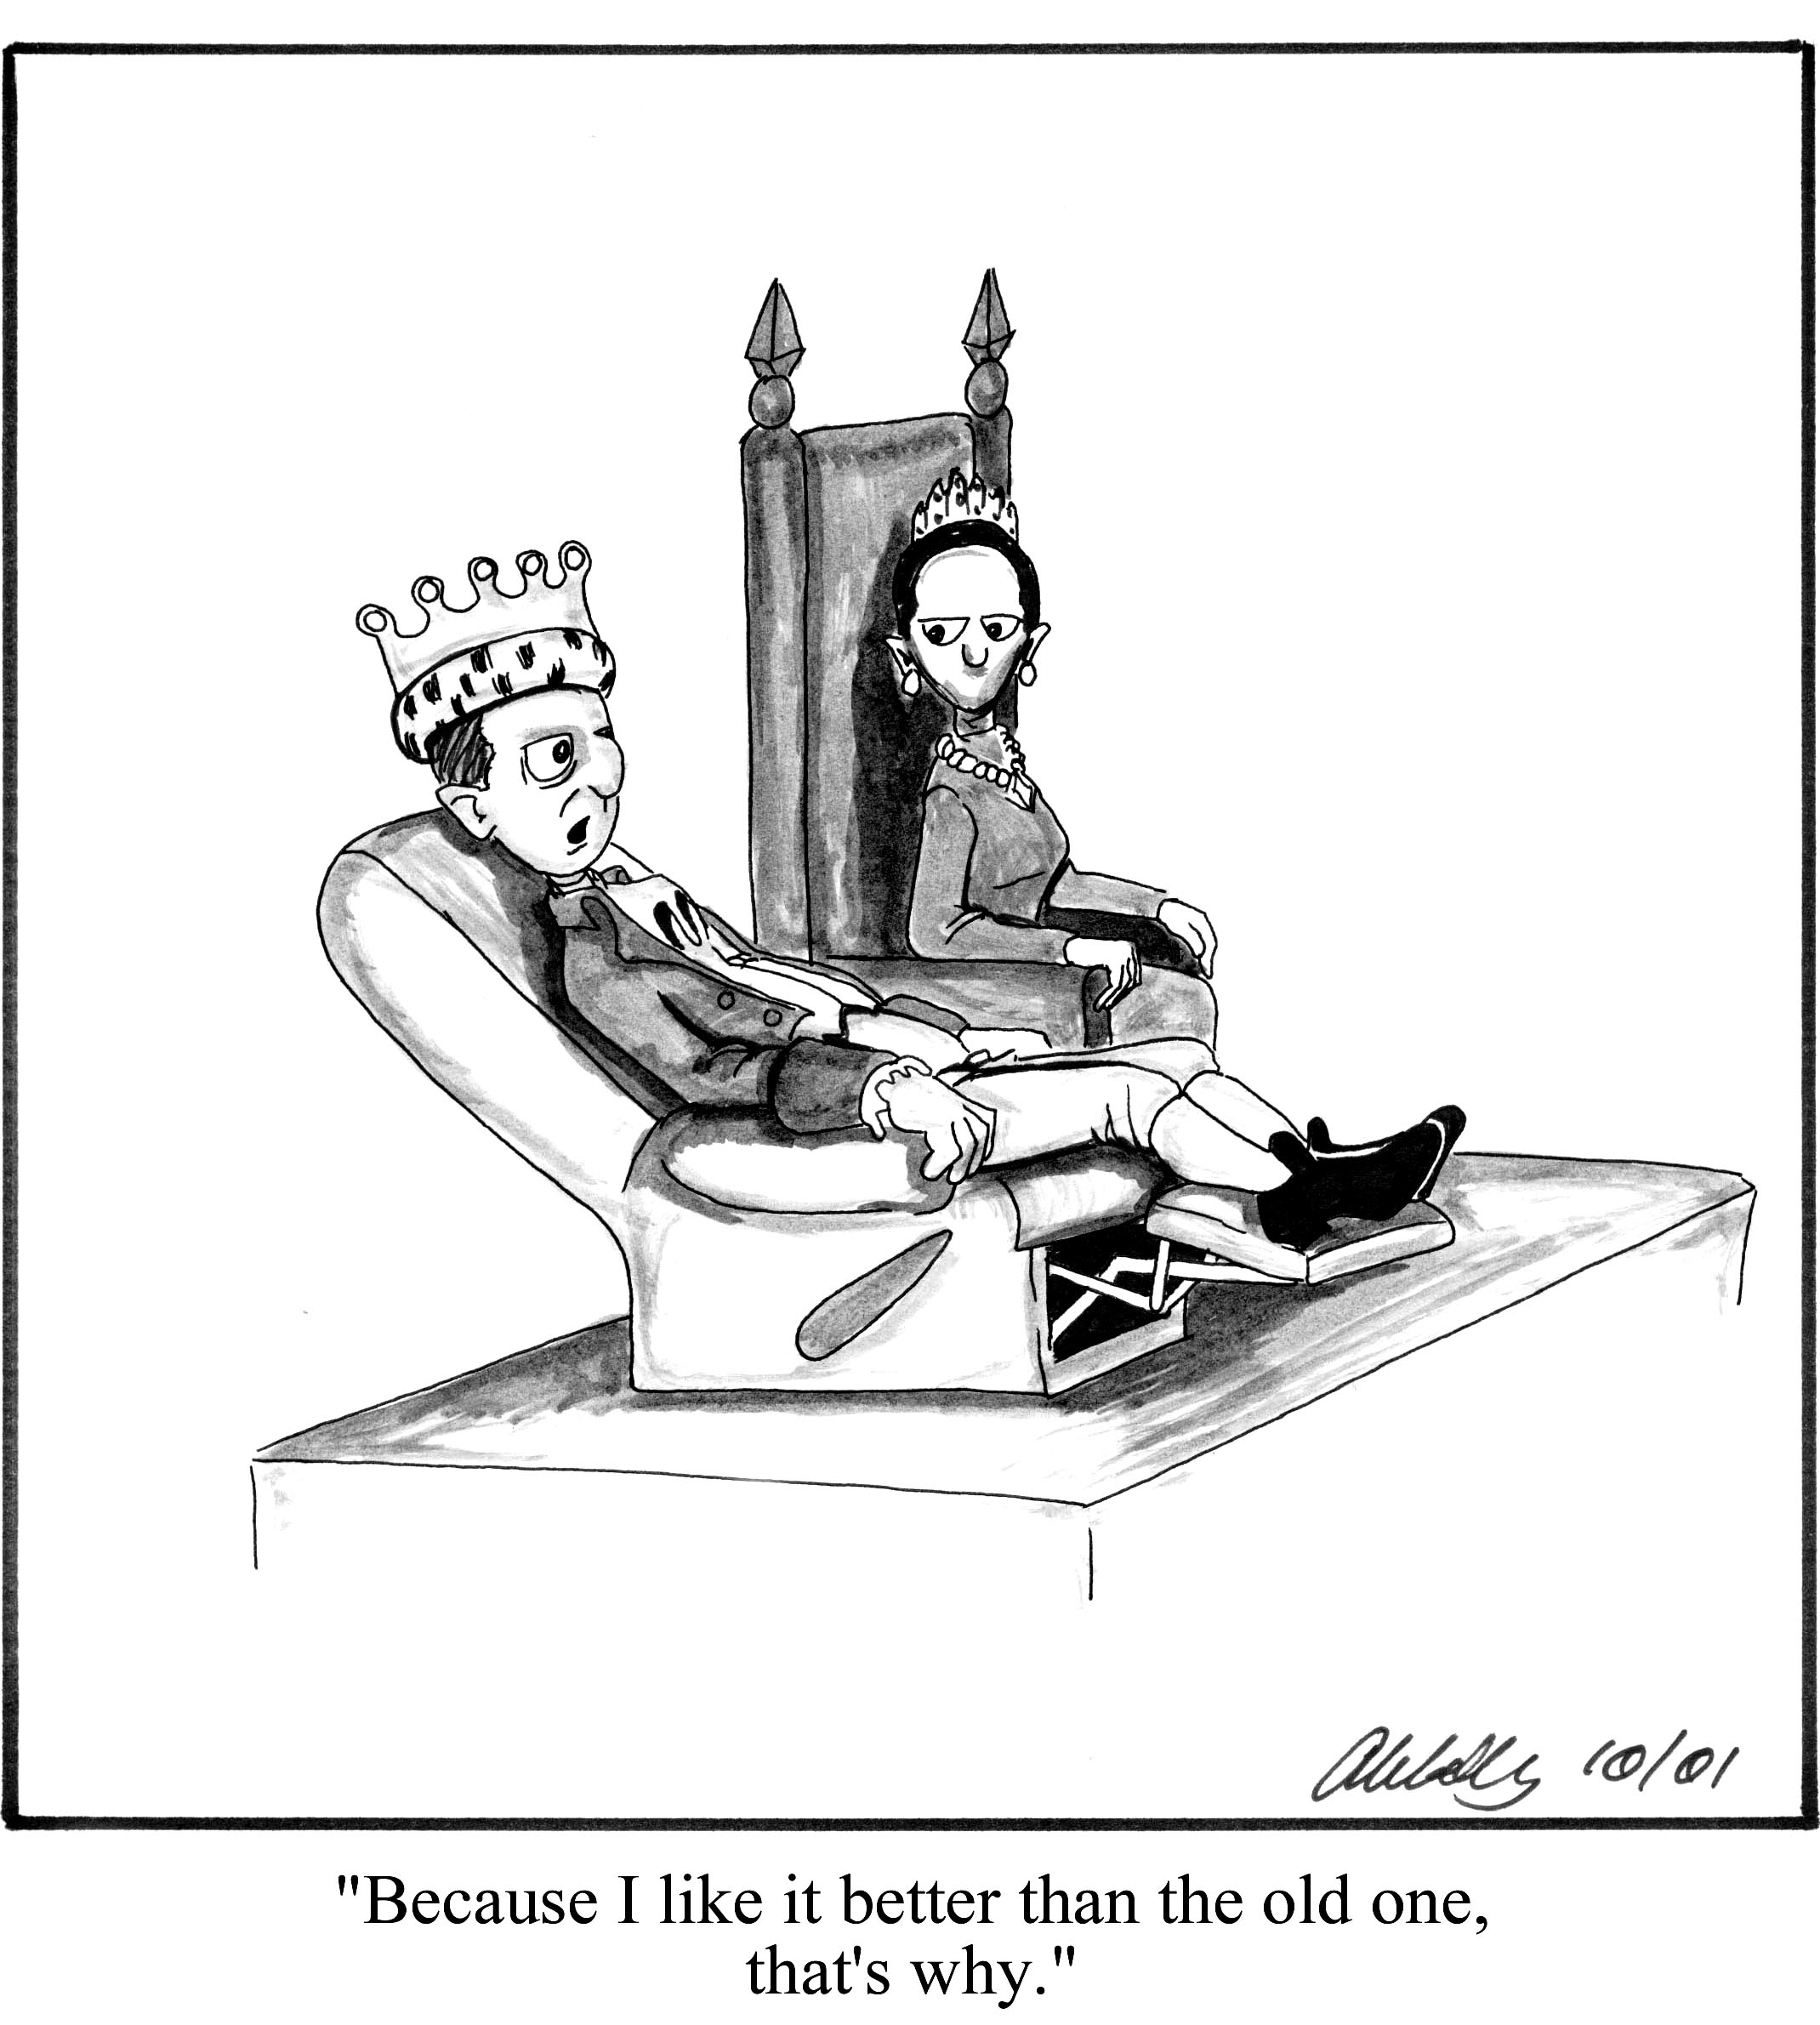
\includegraphics[width=0.15\textwidth]{throneEC.jpg}
%   \end{centering}
%   \caption{Why one should use EasyChair}
%   \label{fig:easythrone}
% \end{figure}

%------------------------------------------------------------------------------
\section{Acknowledgments}
\label{sect:acks}


\label{sect:bib}
\bibliographystyle{plain}
%\bibliographystyle{alpha}
%\bibliographystyle{unsrt}
%\bibliographystyle{abbrv}
\bibliography{easychair}

%------------------------------------------------------------------------------

%------------------------------------------------------------------------------
% Index
%\printindex

%------------------------------------------------------------------------------
\end{document}

